
% Just compile this file using pdflatex after making all required changes.

\documentclass[12pt,a4paper]{report}
\usepackage[pdftex]{graphicx} %for embedding images
\renewcommand{\baselinestretch}{1.5}
%\usepackage{url} %for proper url entries
\usepackage[bookmarks, colorlinks=false, pdfborder={0 0 0}, pdftitle={<pdf title here>}, pdfauthor={<author's name here>}, pdfsubject={<subject here>}, pdfkeywords={<keywords here>}]{hyperref} %for creating links in the pdf version and other additional pdf attributes, no effect on the printed document
%\usepackage[final]{pdfpages} %for embedding another pdf, remove if not required
\usepackage{geometry}
\usepackage[pdftex]{graphicx}
\usepackage{graphicx}
\usepackage{amsmath}
\usepackage{fixltx2e}
\usepackage{multirow}
\usepackage{textcomp}

\geometry{
	left=2.2cm,
	top=2.54cm,
	bottom=2.921cm,
	right=1.5cm
}
\usepackage{fancyhdr}
\pagestyle{fancy}
\lhead{}
\chead{}
\lfoot{\textit{Department of Computer Applications, CET}}
\cfoot{}
\rfoot{\thepage}
\renewcommand{\headrulewidth}{0.4pt}
\renewcommand{\footrulewidth}{0.4pt}

\begin{document}
\renewcommand\bibname{Bibliography} %Renames "Bibliography" to "References" on ref page

%include other pages
\begin{titlepage}
\begin{center}
\textbf{ A  }\\
\vspace{0.35cm}
\textbf{ Seminar Report}\\
\vspace{0.55cm}

\textbf{\Large{Comparison and Performance Analysis of Standard and LVM Based Disk Parititioning}}\\
\vspace{0.2cm}

\normalsize
\vspace{0.5cm}
\emph{Submitted in partial fulfillment of the requirements for the Award of the Degree}\\
\vspace{0.35cm}

\emph{of}\\
\vspace{0.35cm}
Master of Computer Applications\\
\vspace{0.35cm}

\emph{of}\\
\vspace{0.35cm}

\emph{ {APJ Abdul Kalam Technological University} }\\
\normalsize
\vspace{0.5cm}


\includegraphics[height=0.30\textwidth]{./logo}\\
\vspace{0.3cm}

Submitted by\\
\vspace{0.3cm}
\textbf{ASWIN BABU K}\\
\vspace{0.5cm}
\textbf{RegNo: TVE16MCA14}\\
\vspace{1.8cm}

\normalsize
\textbf{Department of Computer Applications}\\[0.3cm]
\textbf{COLLEGE OF ENGINEERING TRIVANDRUM}\\[0.4cm]
\textbf{AUGUST 2018}\\
\end{center}
\end{titlepage}


\begin{titlepage}
\begin{center}
\textbf{DEPARTMENT OF COMPUTER APPLICATIONS}\\[0.5cm]
\textbf{ COLLEGE OF ENGINEERING TRIVANDRUM}\\
[0.5cm]
\vspace{1.2cm}


\includegraphics[width=0.30\textwidth]{./logo}\\
\vspace{0.8cm}
\textbf{CERTIFICATE}\\
\end{center}

\emph{Certified that this Seminar report entitled,
\textbf{``Comparison and Performance Analysis of Standard and LVM Based Disk
Partitioning"} is the paper presented by \textbf{``Aswin Babu K"
(Reg No: TVE16MCA14)} in partial fulfillment of the requirements for the award
of the degree of Master of Computer Applications of APJ Abdul Kalam
Technological University during the year 2018.}\\\\\\\\
\vspace{0.5cm}

Prof. Baby Syla L \hspace{9.5cm} Prof. Jose T Joseph\\ 

\textbf{Co-ordinator}
\hspace{8.9cm} \textbf{Head of the Department}

\end{titlepage}

\begin{titlepage}
\begin{center}
\textbf{\LARGE{Acknowledgement}}\\[0.5cm] 
\end{center}
\paragraph{}
First and for most I thank \textbf{GOD} almighty and to my parents for the success of this seminar. I owe a sincere gratitude and heart full thanks to everyone who shared their precious time and knowledge for the successful completion of my seminar.

I would like to thank \textbf{Dr.Hari V.S}, Principal,  College of Engineering Trivandrum, who helped me during the entire process of work.

I am extremely grateful to \textbf{Prof.Jose T Joseph}, HOD, Dept of Computer Applications, for providing me with best facilities and atmosphere for the creative work guidance and encouragement.

I would like to thank my coordinator,\textbf{ Prof. Baby Syla}, Dept of Computer Applications, who motivated me throughout the work of my seminar.  

I profusely thank other Asst. Professors in the department and all other staffs of CET, for their guidance and inspirations throughout my course of study.

I owe my thanks to my friends and all others who have directly or indirectly helped me in the successful completion of this seminar. No words can express my humble gratitude to my beloved parents and relatives who have been guiding me in all walks of my journey.\\

 \vspace{1.1cm}
\hspace{345pt} \textbf{Abhilash Thankachan}


\end{titlepage}


\begin{titlepage}
\begin{center}
\textbf{\LARGE{Abstract}}\\[1cm]
\end{center}
\normalsize

In the course of twenty five years, Linux has gone from being a hobbyist toy
Operating System run on the creator's 386 machine to an OS that runs everything
from smart watches to Supercomputers. From managing Hard Disk drives having a
few hundred megabytes of storage, current Linux systems are tasked with
management of vast storage arrays, whose size can go up to tens of Petabytes.
From the advent of modern storage devices, disk partitioning was seen as a
necessity, as it allowed proper allocation of storage resources for various
users and services of the system. But traditional disk partitioning has
struggled to keep up with the exhilarating advancements in the field of storage.
Logical Volume Manager or LVM is Linux's answer for easing the storage
management. It does this by further abstracting the storage partitions allowing
them to span multiple physical disks and to be resized even while being mounted.
The seminar introduces standard and LVM based partitioning methods and then
looks if LVM can be used as a replacement for the standard partitioning methods.

\end{titlepage}


\pagenumbering{roman} %numbering before main content starts
\tableofcontents
\listoffigures
\listoftables
%
\newpage
\pagenumbering{arabic} %reset numbering to normal for the main content


\chapter{Introduction }
\paragraph{} The utilized security procedure should likewise consider the improvement of the information recovery time. The DROPS (Division and Replication of Data in the Cloud
for Optimal Performance and Security) technique that aggregately approaches the security
and performance issues. In the DROPS technique, separate a document into sections, and
duplicate the divided information over the cloud nodes. Security is one of the most crucial
aspects among those prohibiting the wide- spread adoption of cloud computing. Cloud se-
curity issues may stem due to the core technology’s implementation (virtual machine (VM)
escape, session riding, etc.), cloud service offerings (structured query language injection,
weak authentication schemes, etc.), and arising from cloud characteristics (data recovery
vulnerability, Internet protocol vulnerability, etc.). For a cloud to be secure, all of the
participating entities must be secure. In any given system with multiple units, the highest
level of the system’s security is equal to the security level of the weakest entity.

 Therefore,
in a cloud, the security benefit does not solely depend on an individual’s security measures.
The neighbouring entities may provide an opportunity to an attacker to bypass the users
defences. The off-site data storage cloud utility requires users to move data in cloud’s
virtualized and shared environment that may result in various security concerns. Pooling
and elasticity of a cloud, allows the physical resources to be shared among many users.
Furthermore, the shared resources may be reassigned to other users at some instance of
time that may result in data compromise through data recovery methodologies. Further-
more, a multi-tenant virtualized environment may result in a VM to escape the bounds
of virtual machine monitor (VMM). The escaped VM can interfere with other VMs may
access to unauthorized data. Similarly, cross-tenant virtualized network access may also
compromise data privacy and integrity. Due to improper media sanitization can also leak
customer’s private data.
\chapter{Related Work}
\paragraph{}Juels et the author of the paper `` New approaches to security and
availability for cloud data,Communications of the ACM '', Vol.
56, No. 2, 2013, pp. 64-73  presented a technique to ensure the
integrity, freshness, and availability of data in a cloud.
The data migration to the cloud is performed by the
Iris file system. A gateway application is designed
and employed in the organization that ensures the
integrity and freshness of the data using a Merkle
tree. The file blocks, MAC codes, and version numbers
are stored at various levels of the tree. The proposed
technique in the paper heavily depends on the user ′ s em-
ployed scheme for data confidentiality. Moreover, the
probable amount of loss in case of data tempering as a
result of intrusion or access by other VMs cannot be
decreased. Our proposed strategy does not depend
on the traditional cryptographic techniques for data
security. Moreover, the DROPS methodology does
not store the whole file on a single node to avoid
compromise of all of the data in case of successful
attack on the node.
\paragraph{}
The authors  G. Kappes, A. Hatzieleftheriou, and S. V. Anastasiadis, Dike of the paper 
``Virtualization-aware Access Control for Multitenant Filesystems'' University of Ioannina, Greece, approached the virtualized and
multi-tenancy related issues in the cloud storage by
utilizing the consolidated storage and native access
control. The Dike authorization architecture is pro-
posed that combines the native access control and
the tenant name space isolation. The proposed system
is designed and works for object based file systems.
However, the leakage of critical information in case of
improper sanitization and malicious VM is not han-
dled. The DROPS methodology handles the leakage
of critical information by fragmenting data file and
using multiple nodes to store a single file.
\chapter{Existing System Approach}
In existing system data reliability, data availability, and response time are dealt with data replication strategies. However, storing replicas data over a number of nodes increases the attack surface for that particular data.For example, storing m replicas of a file in a cloud instead of one replica increases the probability of a node holding file to be chosen as attack sufferer, from 1/n to m/n where n is the total number of nodes. Existing system was not achieving proper security.
\section{Disadvantages}
\begin{itemize}
	\item   A key factor determining the throughput of a cloud that stores data is the data retrieval time.
	\item   In large-scale systems, the problems of data reliability, data availability, and response time are dealt with data replication strategies.
	\item   However, placing replicas data over a number of nodes increases the attack surface for that particular data.
	\item   Affected on security and performance.  
\end{itemize}
\section{Data Fragmentation}
The security of a large-scale system, such as cloud depends on the security of the
system as a whole and the security of individual nodes. A successful intrusion into a single
node may have severe consequences, not only for data and applications on the victim node,
but also for the other nodes. The data on the victim node may be revealed fully because
of the presence of the whole le. A successful intrusion may be a result of some software or
administrative vulnerability. In case of homogenous systems, the same aw can be utilized
to target other nodes within the system. The success of an attack on the subsequent nodes
will require less effort as compared to the effort on the rst node. Comparatively, more effort
is required for heterogeneous systems. However, compromising a single le will require the
effort to penetrate only a single node. The amount of compromised data can be reduced by
making fragments of a data le and storing them on separate nodes. A successful intrusion
on a single or few nodes will only provide access to a portion of data that might not be of
any signicance. Moreover, if an attacker is uncertain about the locations of the fragments,
the probability of nding fragments on all of the nodes is very low. Consider a cloud with
M nodes and a le with z number of fragments. Let s be the number of successful intrusions
on distinct nodes,\linebreak
such that s > z
\paragraph{}
The probability that s number of victim nodes contain all of the z sites storing the le
fragments ( represented by $P(s,z)$ )is given as:

\[
P(s, z)=
\frac{
	\begin{pmatrix}
	s \\
	z 
	\end{pmatrix}
	\begin{pmatrix}
	M - s \\
	s - z
	\end{pmatrix}
}{\begin{pmatrix}
	M \\
	s
	\end{pmatrix}}
\]
\section{Centrality}
\paragraph{}
The centrality of a node in a graph provides the measure of the relative importance
of a node in the network. The node is important in the network if it:
\newline (a) interconnects more nodes than others,
\newline (b) can be reached easily by other nodes, or 
\newline(c) can reach other nodes easily.
\paragraph{}
The objective of improved retrieval time in replication makes the centrality measures
more important. There are various centrality measures; for instance, closeness centrality,
degree centrality, betweenness centrality, eccentricity centrality, and eigen- vector centrality.
Here only elaborate on the closeness, betweenness, and eccentricity centralities because here
using the aforesaid three centralities in this work.
\subsection{Betweenness Centrality} 
\paragraph{}
The betweenness centrality of a node n is the number of the shortest paths, between
other nodes, passing through n. Formally, the betweenness centrality of any node v in a
network is given as:

\[
C_{b}(\upsilon) = \sum_{ a \ \neq \  \upsilon \ \neq \ b} \frac{\delta_{ab}(\upsilon)}{\delta_{ab}}
\] 

\subsection{Closeness Centrality}
\paragraph{}
A node is said to be closer with respect to all of the other nodes within a network, if
the sum of the distances from all of the other nodes is lower than the sum of the distances
of other candidate nodes from all of the other nodes. The lower the sum of distances from
the other nodes, the more central is the node. Formally, the closeness centrality of a node
v in a network is dened as:
\linebreak
\[
C_{c}(\upsilon) = \frac{N - 1}{ \sum _{ a \neq \upsilon} d(\upsilon, a)}
\]

\paragraph{}
where N is total number of nodes in a network and d(v,a)represents the distance between
node v and node a.
\subsection{Eccentricity}
\paragraph{}
The eccentricity of a node n is the maximum distance to any node from a node n. A
node is more central in the network, if it is less eccentric. Formally, the eccentricity can be
given as:
$$ E(\upsilon_{a}) = max _{b} \ d(\upsilon_{a},\upsilon_{b}) $$
\section{T-Coloring}
\paragraph{}
Consider a graph G=(V,E)and a set T containing non-negative integers including 0.
The T- coloring is a mapping function f from the vertices of V to the set of non-negative
integers, such that f(x)- f(y) is not an element of T, where(x,y) is an element of E. The
mapping function f assigns a color to a vertex. In simple words, the distance between the
colors of the adjacent vertices must not belong to T. Formulated by Hale, the T-coloring
problem for channel assignment assigns channels to the nodes, such that the channels are
separated by a distance to avoid interference.

\chapter{Proposed System}
The proposed system called DROPS(Division and Replication of Data in Cloud for Optimal Performance and Security) jointly approaches the security and performance issues. The proposed DROPS scheme ensures that even in the case of a successful attack, no meaningful information is disclosed to the attacker. The DROPS technique doses not depend on traditional cryptographic techniques for data security. The non-cryptographic nature of the proposed scheme makes it faster to perform the required operations (placement and retrieval) on the data. It make sure a controlled replication of the file fragments,
where each of the fragments is replicated only once for the purpose of improved security.
A cloud storage security scheme jointly deals with the security and performance in terms
of retrieval time.
\section{Advantages}
\begin{itemize}
	\item  Improve security.
	\item  Improve performance. 
	\item  No information is revealed to the attacker. (If an attacker is uncertain about the locations of the fragments, the probability of finding fragments on all of the nodes is very low.)
	\item  No load on single node of cloud.
	\item  Numbers of fragments are decided according to owner’s choice.
\end{itemize}
\chapter{ DROPS System Model}
\paragraph{}
A cloud that consists of M nodes, each with its own storage capacity. Let Si represents
the name of ith node and si denotes total storage capacity of Si Communication time
between Si and Sj is the total time of all of the links within a selected path from Si to Sj
represented by c(i, j). Consider N number of file fragments such that Ok denotes k -th
fragment of a file while ok represents the size of k-th fragment. Pk denote the primary
node that stores the primary copy of Ok, replication scheme for Ok denoted by Rk is also
stored at Pk and Whenever there is an update in not as an independent document. Please
do not revise any of the current designations Ok , the updated version is sent to Pk that
broadcasts the updated version to all of the nodes in Rk. Let colSi store the value of
assigned color to Si. The colSi can have one out of two values, namely: open color and
close color. The value open color represents that the node is available for storing the file
fragment. The value close color shows that the node cannot store the file fragment The
set T is used to restrict the node selection to those nodes that are at hop-distances not
belonging to T.
\paragraph*{}
In the DROPS methodology, not to store the entire file at a single node. The DROPS
methodology fragments the file and makes use of the cloud for replication. The fragments
are distributed such that no node in a cloud holds more than single fragment, so that even
a successful attack on the node leaks no significant information.

\begin{table}
	\begin{center}
		\begin{tabular}{|c|c|} 
			\hline % draw horizontal line
			Symbols & Meanings \\
			\hline
			M & Total number of nodes in the cloud \\
			\hline
			N & Total number of fragments to be placed \\
			\hline
			{$O_k$} & k-th fragment of the file \\
			\hline
			{$o_k$} & Size of {$O_k$} \\
			\hline
			{$S^i$} & i-th node \\
			\hline
			{$s_i$} & Size of {$S^i$}  \\
			\hline
			{$cen_i$} & Centrality measure of {$S^i$} \\
			\hline
			{$col_{S^i}$} & Color assigned to {$S^i$} \\								\hline
			{$r^i_k$} & Number of reads for {$O_k$} from {$S^i$} \\		
			\hline
			{$R^i_k$} & Aggregate read cost of  {$r^i_k$} \\		
			\hline
			{$w^i_k$} & Number of writes for {$O_k$} from {$S^i$} \\
			\hline
			{$W^i_k$} & Aggregate write cost of  {$w^i_k$} \\
			\hline
			{$N N^i_k$} & Nearest neighbour of {$S^i$} holding{$O_k$} \\
			\hline
			c(i,j) & Communication cost between {$S^i$} and {$S^j$} \\
			\hline
			{$P_k$} & Primary node for {$O_k$} \\
			\hline
			{$R_k$} & Replication schema for {$O_k$} \\
			\hline
			RT & Replication Time \\
			\hline
			
		\end{tabular}
		\caption{Notations and their meanings.}
	\end{center}
\end{table}

%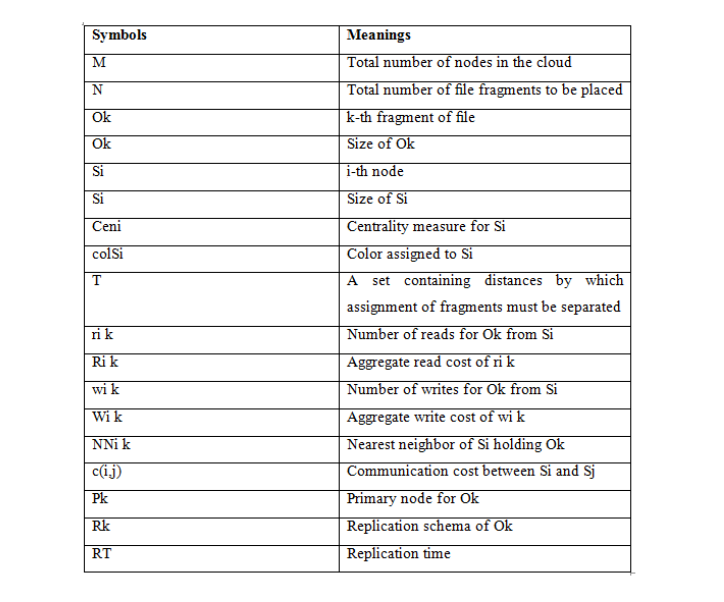
\includegraphics[scale=0.65]{meaningtable}

\paragraph*{}
\newpage
In the DROPS methodology, user sends the data file to cloud. The cloud manager
system(a user facing server in the cloud that entertains user’s requests) upon receiving the file performs:

\begin{enumerate}
	\item fragmentation
	\item first cycle of nodes selection and stores one fragment over each of the selected node and
	\item second cycle of nodes selection for fragments replication. The cloud manager keeps
	record of the fragment placement and is assumed to be a secure entity.
\end{enumerate}

\chapter{ DROPS Architecture}

This system mainly consist of 3 modules:
\begin{figure}
	\centering
	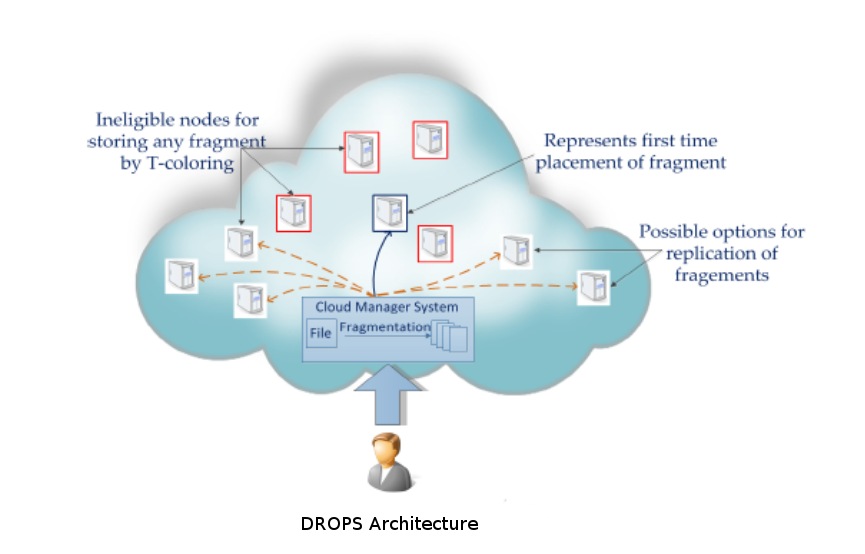
\includegraphics[width=0.95\textwidth]{./droparchitecture.png}
	\caption{DROPS Architecture}
\end{figure}
\section{Cloud Client}
\paragraph*{} 
Cloud client should be Data owner or Data user.
\subsection{Data Owner}
\paragraph*{}
Data owner is responsible for uploading file on cloud as well as view files uploaded by him or others. Data owner has information about the placed fragment and its replicas with their node numbers in cloud. 
\subsection{Data User}
\paragraph*{}
Data user is the one who is responsible for downloading files or view files uploaded by others. To download file from cloud he has to be authenticated user otherwise he will be considered as attacker.
\section{Cloud Server}
\subsection{Fragmentation}
\paragraph*{}
This approach is used for fragmenting the file for security purpose at sever side. This approach runs the Fragmentation algorithm. It has file as input and produces the file fragments as output.

\subsection{Replication}
\paragraph*{}
This approach creates replicas (duplicate copy) of fragments. These replicas are useful
when one of fragment is corrupted by attacker then to provide file for user admin replaces
its replica at that place and combine all fragments and send file to authenticated user or
data owner. To make replicas of file fragments this approach runs replication algorithm
which takes input as fragments and produces its replicas as output.

\subsection{Allocation}
\paragraph*{}
After the file is spitted and replicas are generated then allocate that fragments at
cloud server for storing data. While storing or allocating that fragments, consider security
issues. So the proposed method using T- Coloring Graph concept for placing fragments
at different nodes on cloud server. This approach runs Fragment allocation algorithm
which takes input as fragments and produces the output as fragments allocated with node
numbers.

\section{Admin}
\paragraph*{} 
Admin is an authorized person who has rights to validate authorized data owner
and user. He is also responsible for allocation of block and maintains information and
authentication.
\section{Fragment Placement}
\paragraph*{}
In the DROPS methodology, not to store the entire le at a single node. The DROPS
methodology fragments the le and makes use of the cloud for replication. The fragments
are distributed such that no node in a cloud holds more than a single fragment, so that even
a successful attack on the node leaks no signicant information. The DROPS methodology
uses controlled replication where each of the fragments is replicated only once in the cloud
to improve the security. Although, the controlled replication does not improve the retrieval
time to the level of full-scale replication, it signicantly improves the security.The fragment placement strategy is presented in
the algorithm given below.
\\
\begin{figure}
	\centering
	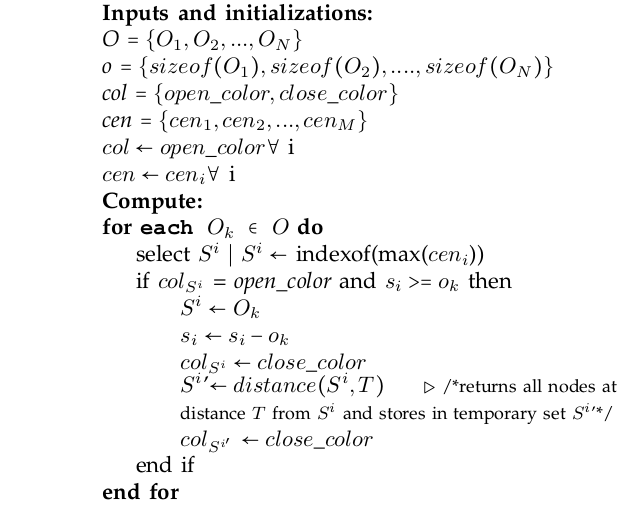
\includegraphics[scale=0.5]{placementalgo}
%	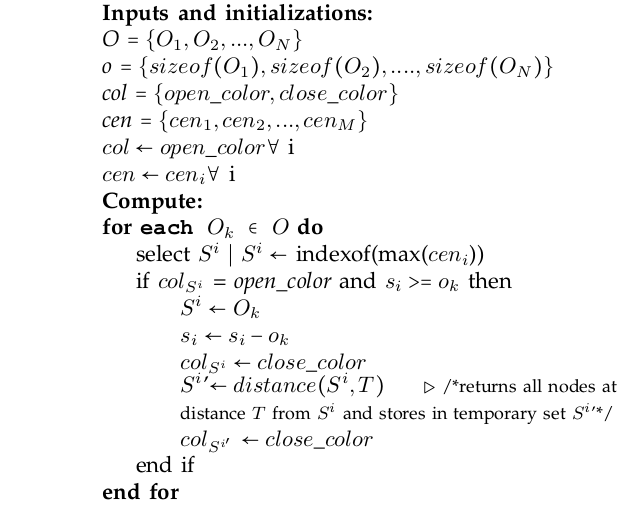
\includegraphics[width=0.9\textwidth]{./placementalgo.jpg}
	\caption{Algorithm for Fragment Placement}
\end{figure}

\paragraph*{}

Initially, all of the nodes are given the open color. Once a fragment is placed on the
node, all of the nodes within the neighborhood at a distance belonging to T are assigned
close color. In the aforesaid process, lose some of the central nodes that may increase the
retrieval time but achieve a higher security level. If somehow the intruder compromises
a node and obtains a fragment, then the location of the other fragments cannot be de-
termined. The attacker can only keep on guessing the location of the other fragments.
However,the probability of a successful coordinated attack is extremely minute. The pro-
cess is repeated until all of the fragments are placed at the nodes. The above algorithm
represents the fragment placement methodology.
\section{Fragment Replication}
\paragraph*{}
In addition to placing the fragments on the central nodes, this approach also per-
form a controlled replication to increase the data availability, reliability, and improve data
retrieval time. Place the fragment on the node that provides the decreased access cost
with an objective to improve retrieval time for accessing the fragments for reconstruction
of original le. While replicating the fragment, the separation of fragments as explained in
the placement technique through T- coloring, is also taken care off.
\paragraph*{}
In case of a large number of fragments or small number of nodes, it is also possible
that some of the fragments are left without being replicated because of the T-coloring.
As discussed previously, T-coloring prohibits to store the fragment in neighborhood of a
node storing a fragment, resulting in the elimination of a number of nodes to be used for
storage. In such a case, only for the remaining fragments, the nodes that are not holding
any fragment are selected for storage randomly. The replication strategy is presented in
the algorithm given below.
\begin{figure}
	\centering
	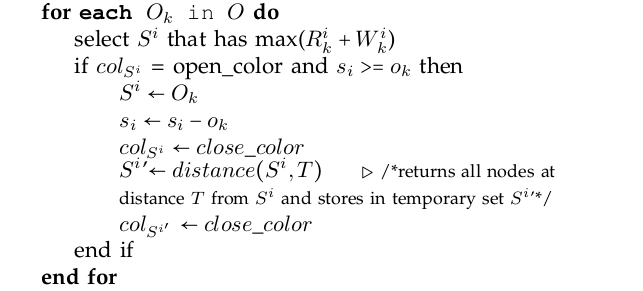
\includegraphics[scale=0.5]{replicationalgo}
	\caption{Algorithm for Fragment Replication}
\end{figure}
\section{Replication Time}
\paragraph*{}
Aim is to minimize the overall total network transfer time or replication time (RT)
or also termed as replication cost (RC). The RT is composed of two factors: (a) time due
to read requests and (b) time due to write requests.

\begin{itemize}
	\item The total read time of Ok by Si from NNi k is denoted by Ri k and is given by:
	$$ R_{k}^{i} = r_{k}^{i}o_{k}c(i , N N_{k}^{i})$$
	\item The total time due to the writing of Ok by Si ad- dressed to the Pk is represented as Wi
	k and is given:
	\[
	W_{k}^{i} = w_{k}^{i}o_{k}(c(i, P_{k})+ \sum_{ (j \in\neq R_{k}) , j \neq i} c(P_{k}, j))
	\]
	\item The overall RT is represented by:
	\[
	RT = \sum_{i = 1}^{M} \sum_{ k = 1}^{N} (R_{k}^{i} + W_{k}^{i})
	\]
	\item The storage capacity constraint states that a file fragment can only be assigned to a
	node, if storage capacity of the node is greater or equal to the size of fragment.
	\item To handle the download request from user, the cloud manager collects all the fragments from the nodes and reassemble them into a single file. Afterwards, the file is sent to the
	user.
\end{itemize}
\section{Features of DROPS}
\begin{itemize}
	\item It ensures that even in case of a successful attack, no meaningful information is revealed
	to the attacker.
	\item A successful attack on a single node must not reveal the locations of other fragments
	within the cloud.
	\item The nodes storing the fragments, are separated with certain distance by means of graph
	T-coloring to prohibit an attacker of guessing the locations of the fragments.
	\item Does not rely on the traditional cryptographic techniques for the data security.
	\item Faster
	\item Higher level of security with slight performance overhead.
\end{itemize}
\chapter{Conclusion and Future Scope}
Though the Logical Volume Manager is a fairly complex storage system, it has
been engineered to provide performance figures similar to the ones provided by
traditional partitioning.\\ 

LVM is easy to setup, is practically free and provides a number of features such
as convinient backups through snapshots, easy resizing of partitions and
improved performance using striped volumes while providing satisfactory
performance. The study concluded that LVM is capable of being a viable
replacement to traditional partitioning in both server and development
environments.\\ 

Capacity and performance of computer storage continues to increase, while need
for higher storage capacities continues to increase at a greater rate. LVM's
importance will continue to increase as big data and deep learning technolgies
become commonplace. Further, greater read/write speeds will bring the
performance difference between native and LVM disk performance to a point in
which they are hardly relevant anymore. In short, LVM has the potential to be
the de-facto standard for Linux storage and it seems to be moving aggresively
towards reaching the goal.

\begin{thebibliography}{99}

\bibitem{1}
    Milivoj Boznic, Milos Djukic, Dragan Narancic, Istvan Pap,
    \textit{``Comparison and Analysis of Standard disk Partitioning and LVM
    based disk Partitioning on Linux Systems''}, TELSIKS 2017

\bibitem{2}
    Borislav Djordjevic, Valentina Timcenko
    \textit{``LVM in the Linux Environment: Performance Examination''},
    Tehnicki Vjesnik, October 2015

\bibitem{3}
    Prashanth Nayank, Robert Ricci
    \textit{``Detailed Study on Linux Logical Volume Manager''},
    Flux Research Group, August 2013

\bibitem{4}
    David A Patterson, Garth Gibson, Randy H Katz
    \textit{``A Case for Redundant Array of Inexpensive Disks (RAID)''},
    SIGMOD '88, June 1988 

\end{thebibliography}




\end{document}
\grid
